



\documentclass[]{article}

\usepackage{indentfirst}
\usepackage{cmap}					% поиск в PDF
%\usepackage[T2A]{fontenc}			% кодировка
%\usepackage[utf8]{inputenc}			% кодировка исходного текста
\usepackage[english,russian]{babel}	% локализация и переносы
\usepackage{amsmath, amsfonts, amssymb, amsthm, mathtools}
\usepackage{icomma}
\usepackage{mathrsfs}

\usepackage{graphicx}
\usepackage{ upgreek }
%рисунки и все с ними связанное
\graphicspath{{pic/}}
\setlength\fboxsep{3pt}
\setlength\fboxrule{1pt}

\begin{document}
	
	% НАЧАЛО ТИТУЛЬНОГО ЛИСТА
	\begin{center}
		\hfill \break
		\large{Министерство образования Российской Федерации}\\
		\large{НАЦИОНАЛЬНЫЙ ИССЛЕДОВАТЕЛЬСКИЙ УНИВЕРСИТЕТ}\\ 
		\large{“НИУ МЭИ”}\\
		
		\hfill \break
		\normalsize{Институт радиоэлектроники}\\
		\hfill \break
		\normalsize{Кафедра Радиотехнических систем}\\
		\hfill\break
		\hfill \break
		\hfill \break
		\hfill \break
		\large{Отчет по 
			
			Курсовому проекту
			
			«Разработка модуля расчёта координат спутника ГЛОНАСС»	}\\
		\hfill \break
		\hfill \break
		\hfill \break
		
		\hfill \break
		
		\hfill \break
		
		\hfill \break
		\hfill \break
	\end{center}
	
	\hfill \break
	\hfill \break
	
	\normalsize{ 
		\begin{tabular}{cccc}
			
			
			Руководитель & \underline{\hspace{3cm}}& к.т.н., доцент & Корогодин И.В. \\\\
			
			Исполнитель & \underline{\hspace{3cm}} &студент группы ЭР-15-15 &Волнухина Е.Д. \\\\
		\end{tabular}
	}\\
	\hfill \break
	\hfill \break
	\begin{center} Москва 2020 \end{center}
	\thispagestyle{empty} % выключаем отображение номера для этой страницы
	
	% КОНЕЦ ТИТУЛЬНОГО ЛИСТА
	\tableofcontents
	
	
	\newpage
	\section{Введение}
	Данная работа выполняется студентами 5 курса с целью ознакомления с различными инструментами и техниками используемых при  разработке АП СРНС. Работа делится на три этапа:
	
	1. Использование сторонних средств;
	
	2. Моделирование;
	
	3. Реализация.
	
	Для каждого этапа была получена соответствующая научно-техническая продукция.
	
	Исходные данные: 
	
	На крыше корпуса Е МЭИ установлена трехдиапазонная антенна Harxon HX-CSX601A. Она через 50-метровый кабель, сплиттер, bias-tee и усилитель подключена к трем навигационным приемникам:
	Javad Lexon LGDD, SwiftNavigation Piksi Multi, Clonicus разработки ЛНС МЭИ.
	Приемники осуществляют первичную обработку сигналов, выдавая по интерфейсам соответствующие потоки данных - наблюдения псевдодальностей и эфемериды спутников. 
	
	Номер спутника ГЛОНАСС: 4
	Приемник: Clonicus
	\newpage
	
	\section{Этап 1.Использование сторонних средств}
	\subsection{Задание на этап №1}
	На этапе № 2 необходимо получить:
	
	-Описание процесса использования RTKLIB;
	
	-Эфемериды собственного спутника по данным RTKNAVI из состава;
	
	-RTKLIB (номер спутника ГЛОНАСС см. в журнале выше);
	
	-Эфемериды собственного спутника в gnav-файле RINEX;
	
	-График угла места собственного спутника от времени по данным Trimble GNSS Planning Online на заданный интервал времени (см. задание второго этапа);
	
	-SkyView по данным Trimble GNSS Planning Online на заданный интервал времени (см. задание второго этапа).
	
	Для того чтобы получить эфемериды спутников, воспользуемся пакетом RTKLIB и сервисом gnssplanning. 
	
	\subsection{Работа с  бинарным  файлом}
	Первое, что нужно сделать- скачать из указанного репозитория  файл в формате .bin, который содержит данные с приемника. 
	\subsubsection{Использование RTKNAVI}
	Из указанного репозитория скачиваем папку «RTKLIB\_bin\_master». В открывшейся папке находим приложение «RTKNAVI», рис.\ref{rtknavi} .
	
	\begin{figure}[h!]
		
		\centering{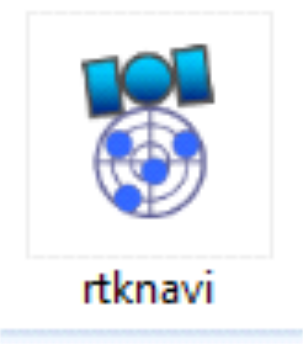
\includegraphics[scale=1]{rtknavi}}
		\caption{Приложение «rtknavi»}
		\label{rtknavi}
	\end{figure}

	В открывшемся окне программы меняем формат времени на GPST (рис.\ref{interf_rtknavi}). Нажимаем кнопку «I» в открывшемся окне ставим галочку рядом с «(1) Rover», и ниже в любую строку «Input File Paths» загружаем файл с данными приемника формата .bin (рис.\ref{interf_rtknavi_2}).
	
		\begin{figure}[h!]
		\centering{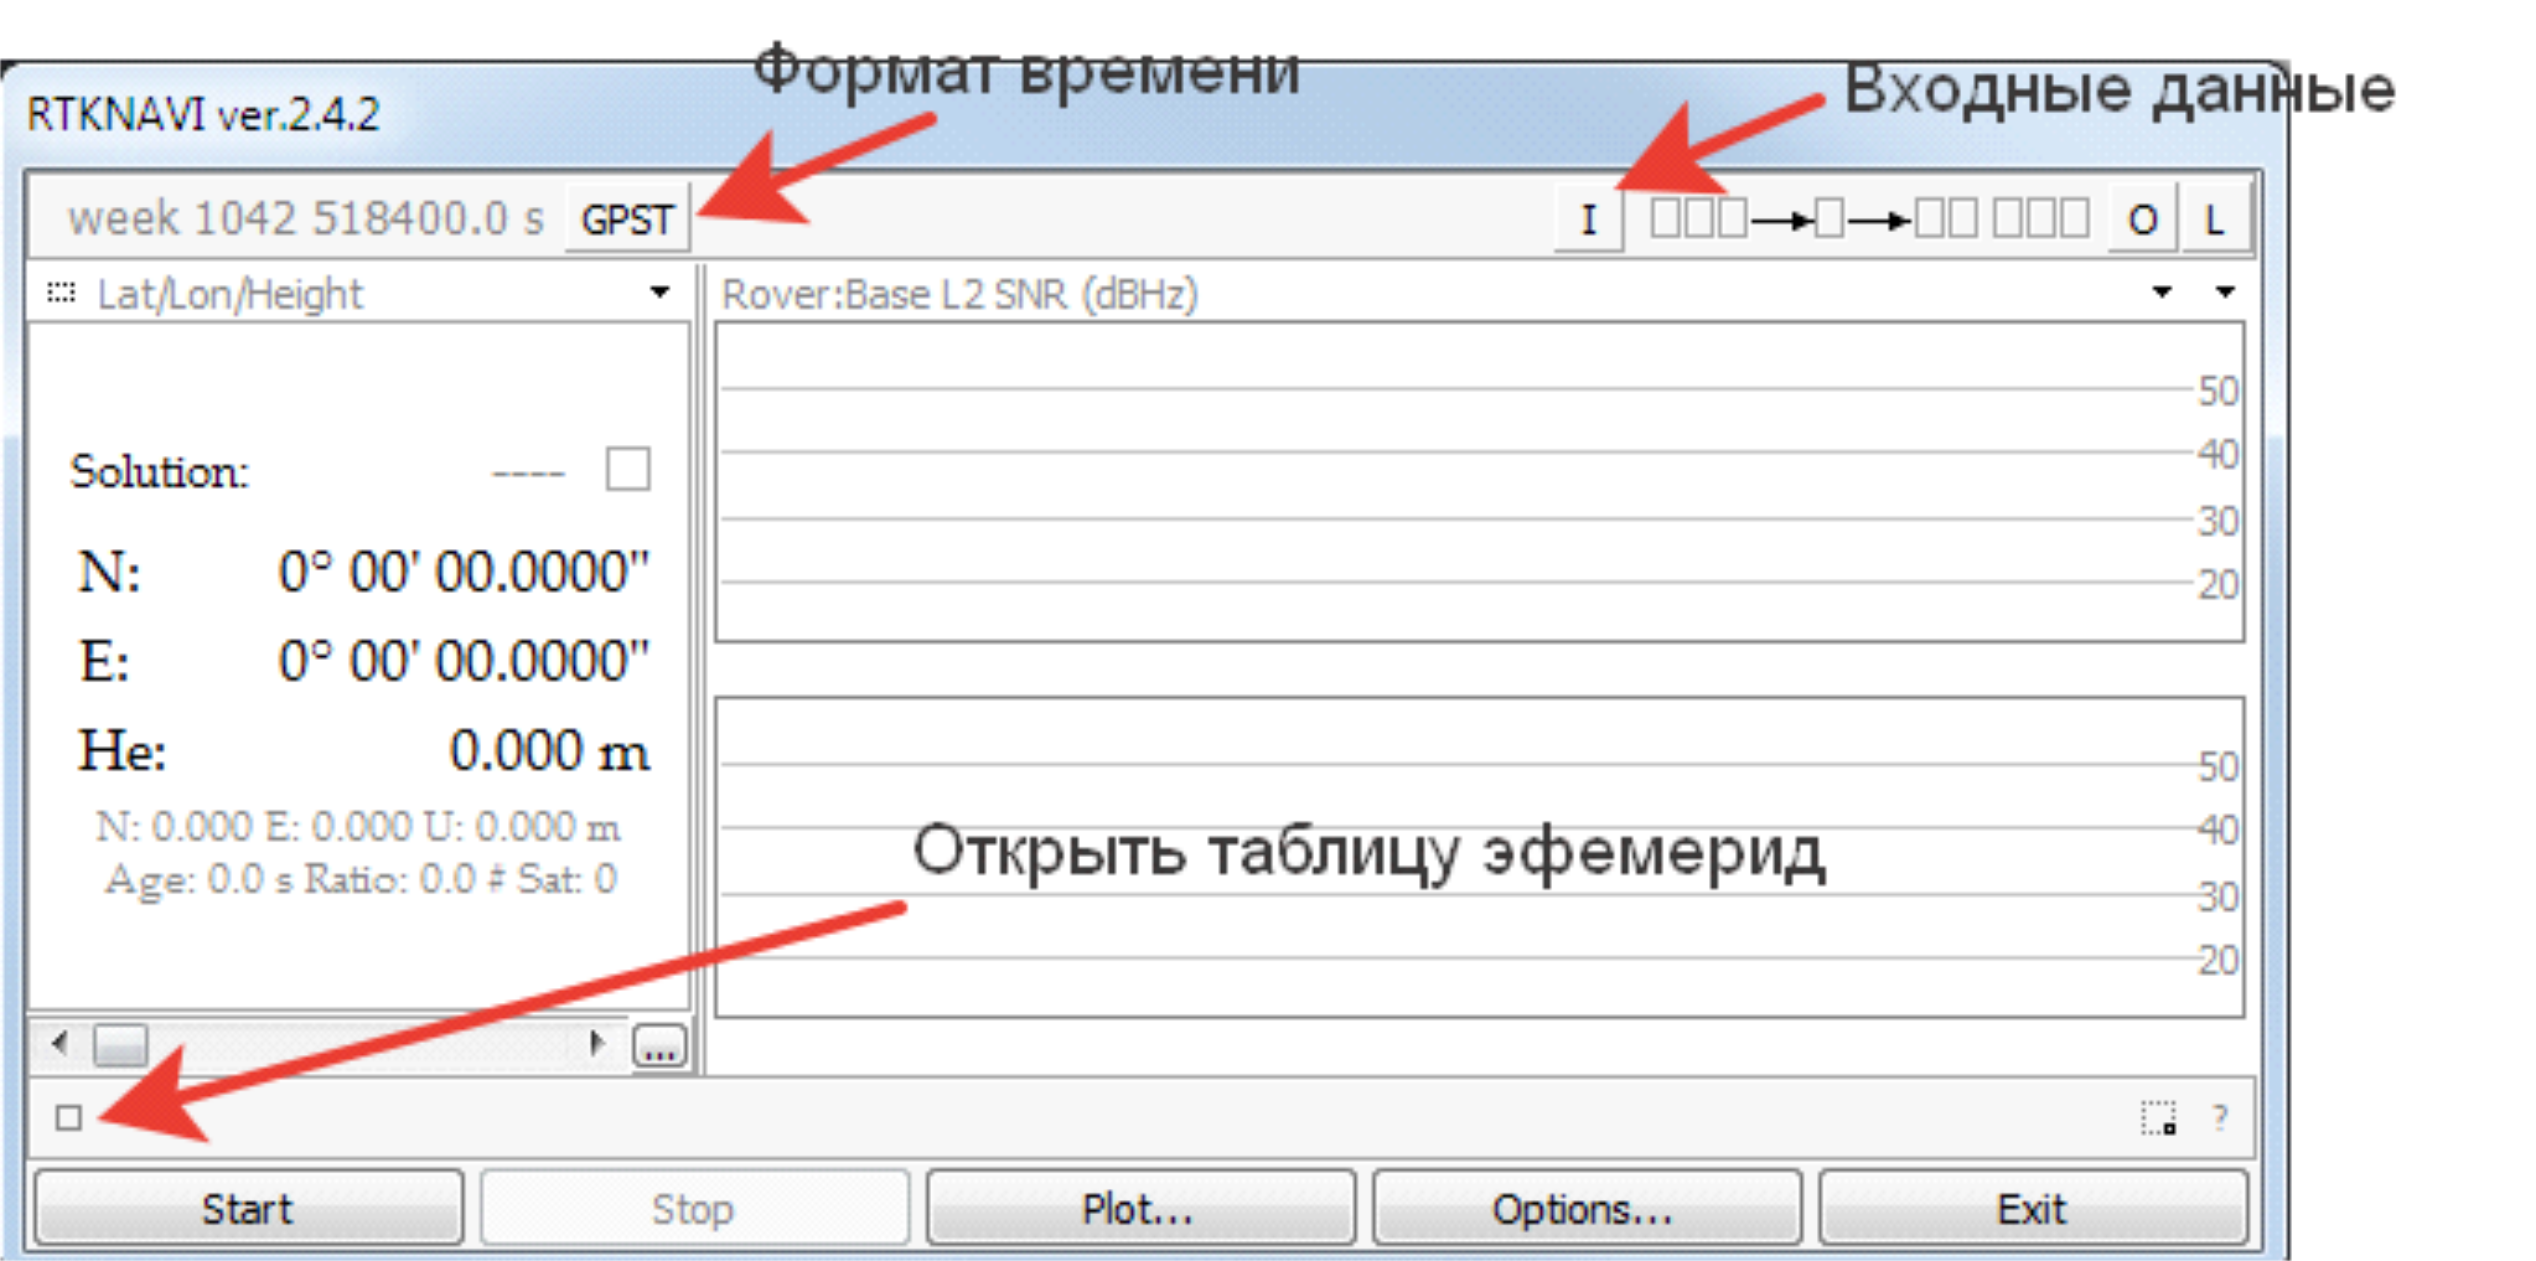
\includegraphics[scale=0.7]{interf_rtknavi}}
		\caption{Интерфейс приложения «rtknavi»}
		\label{interf_rtknavi}
	\end{figure}
	\begin{figure}[h!]
	
	\centering{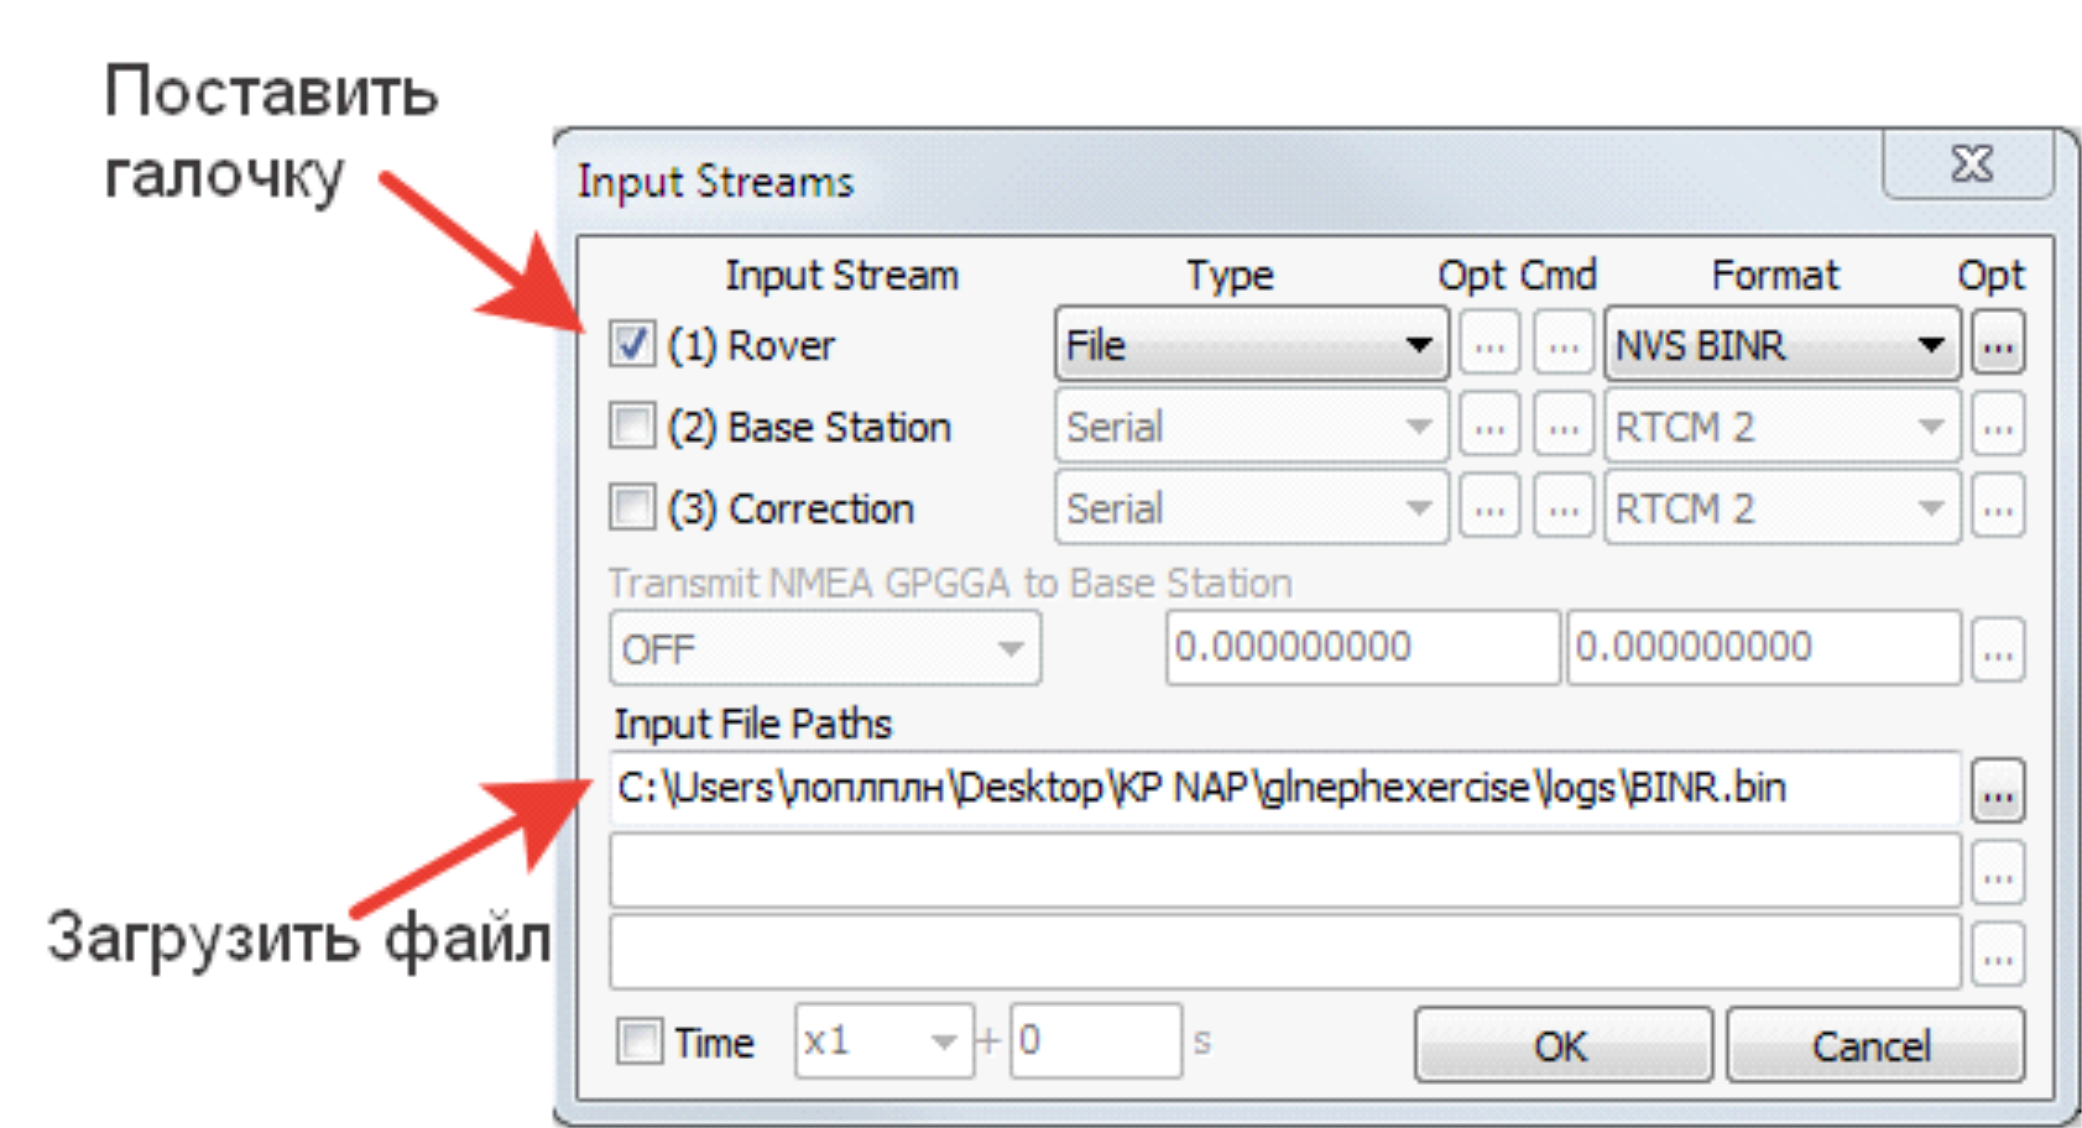
\includegraphics[scale=0.7]{interf_rtknavi_2}}
	\caption{Интерфейс приложения «rtknavi»}
	\label{interf_rtknavi_2}
	\end{figure}
	
	Затем следует нажать небольшую кнопку в левом нижнем углу. В открывшемся окне вместо «RTK» нужно выбрать «Nav GLONASS» (рис.\ref{efem}).
	 \begin{figure}[h!]
	 	
	 	\centering{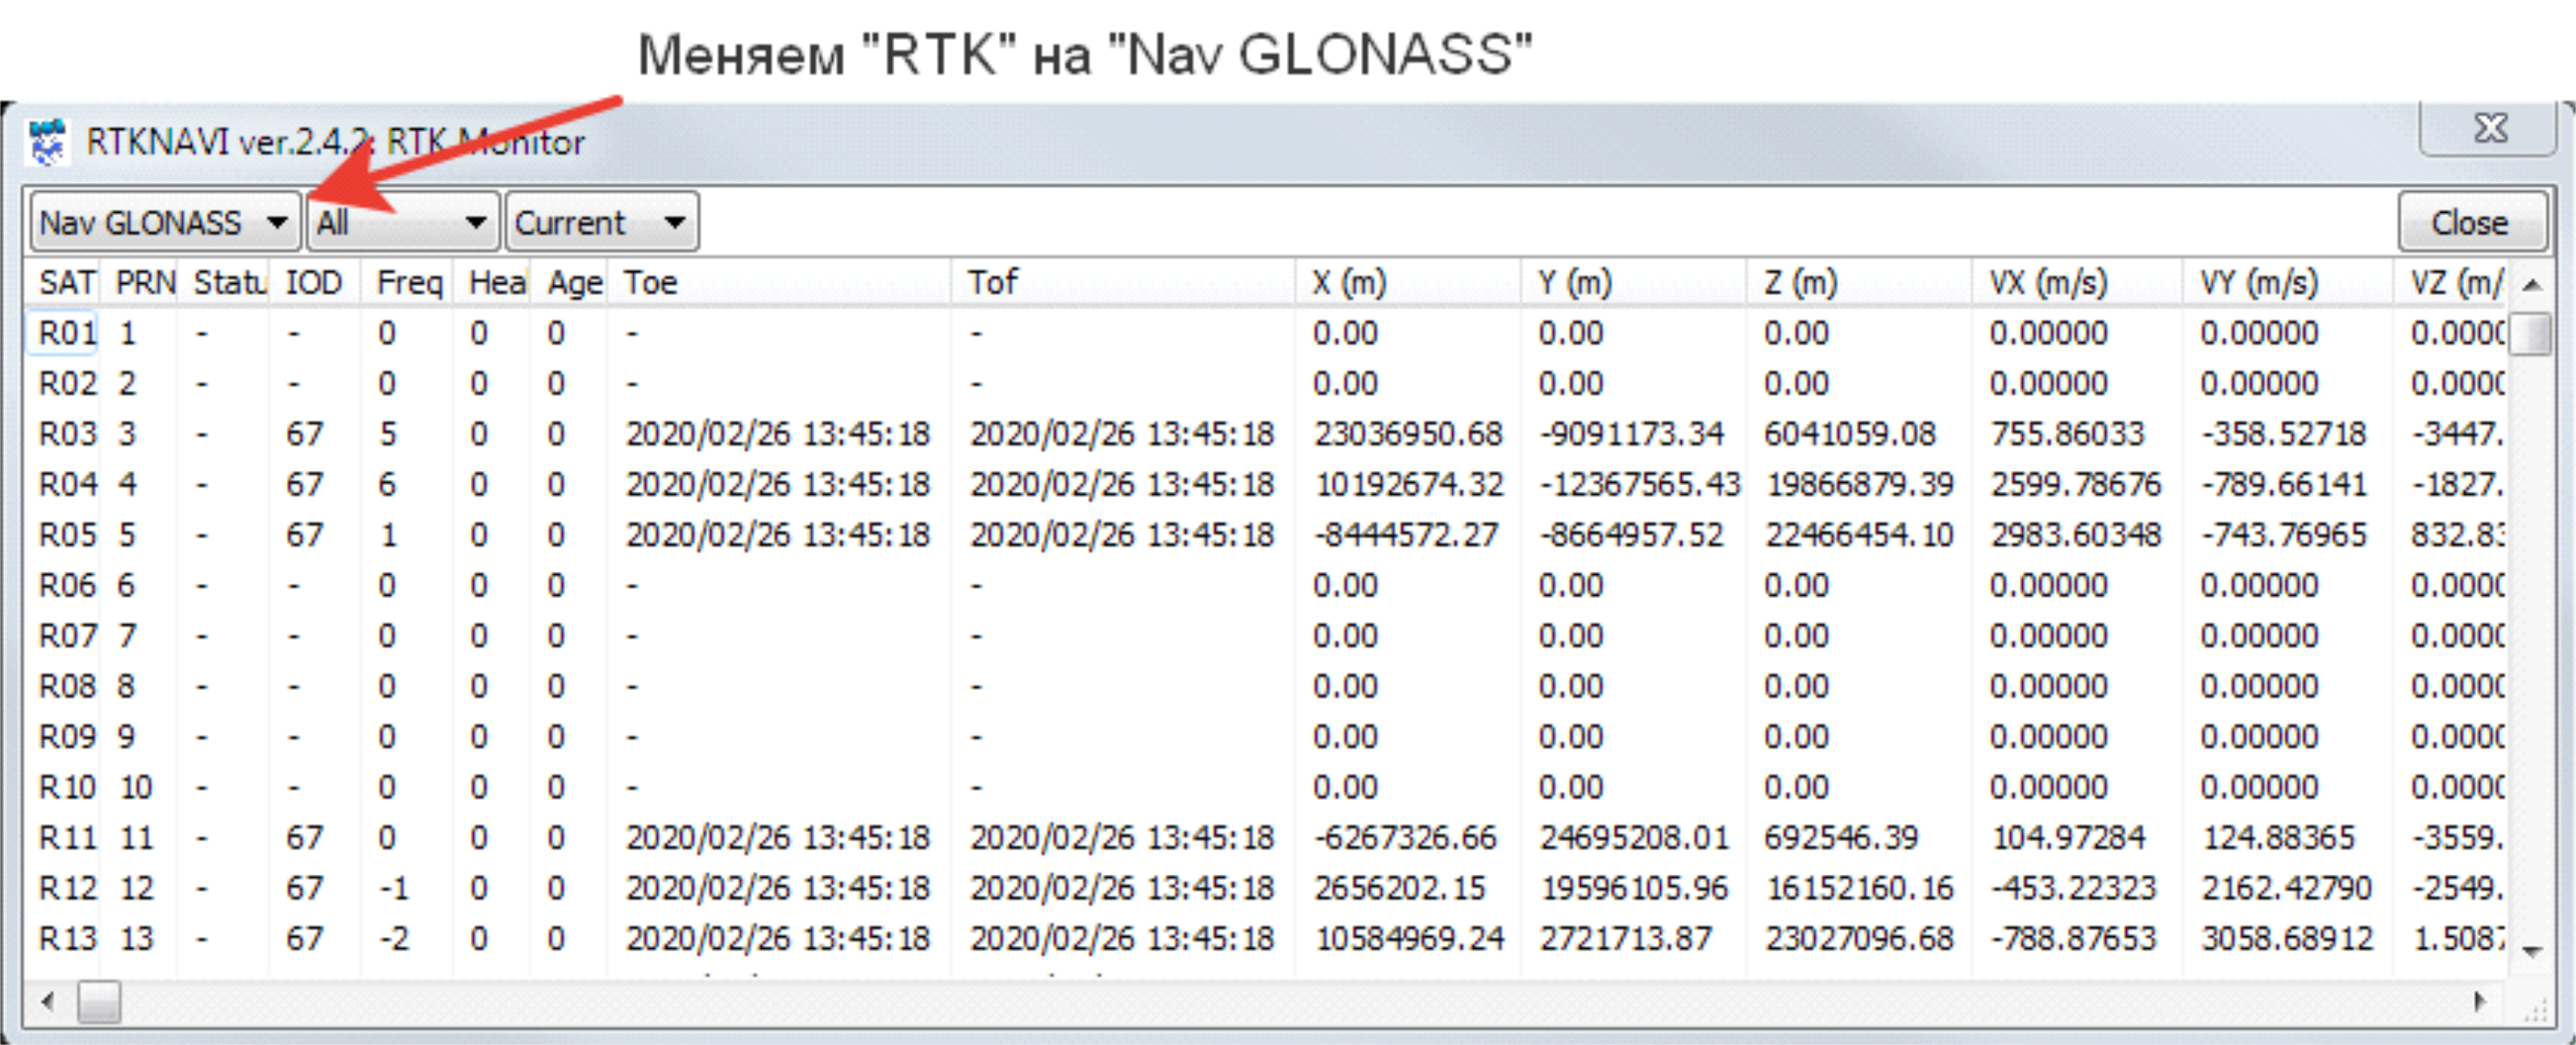
\includegraphics[scale=0.7]{efem}}
	 	\caption{Полученные эфемериды}
	 	\label{efem}
	 \end{figure}
 \newpage
 \subsubsection{Использование rtkconv}
 В папке «RTKLIB\_bin\_master»  находим приложение «rtkconv» (рис.\ref{rtkconv}).
 	\begin{figure}[h!]
 	
 	\centering{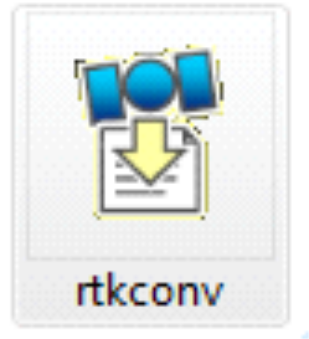
\includegraphics[scale=1]{rtkconv}}
 	\caption{Приложение «rtkconv»}
 	\label{rtkconv}
 \end{figure}

 В строке «RTCM, RCV RAW or RINEX OBS  ?»   нужно указать путь к файлу, который будет обработан (рис.\ref{interf_rtkconv}).
 В строке «Output Directory» нужно выбрать путь к папке, в которую будут записаны выходные данные.
 В списке «Format» требуется  выбрать NVS BINR. После этого нужно нажать кнопку «Convert», и тогда можно получить файл  с эфемеридами ГЛОНАСС в формате .gnav (рис.\ref{efem_2})
 	\begin{figure}[h!]
 	
 	\centering{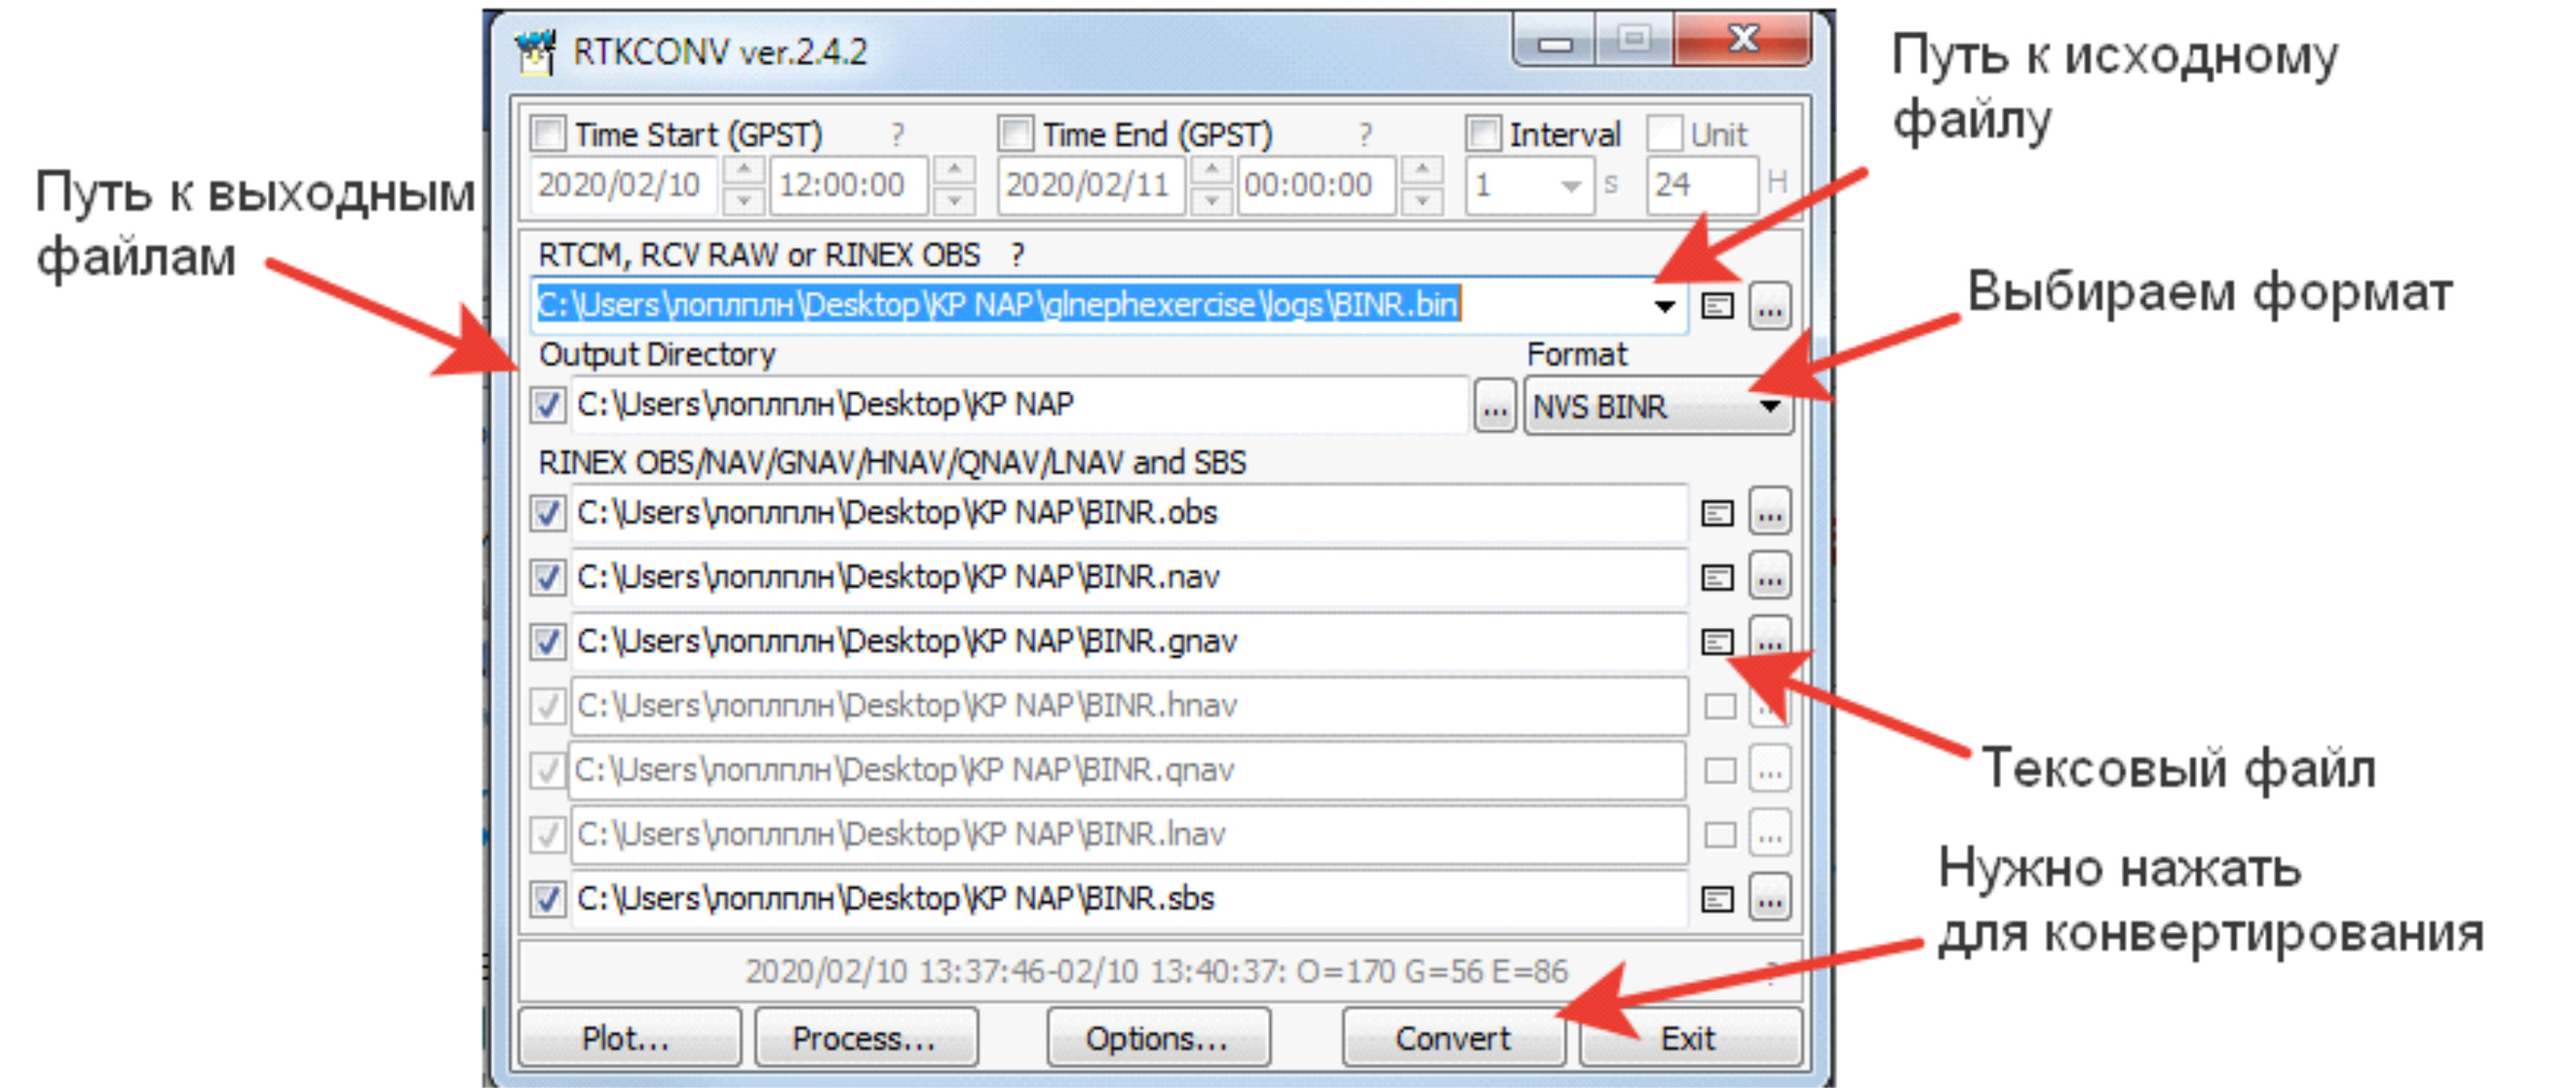
\includegraphics[scale=0.7]{interf_rtkconv}}
 	\caption{Интерфейс приложения «rtkconv»}
 	\label{interf_rtkconv}
 \end{figure}
	\begin{figure}[h!]
	
	\centering{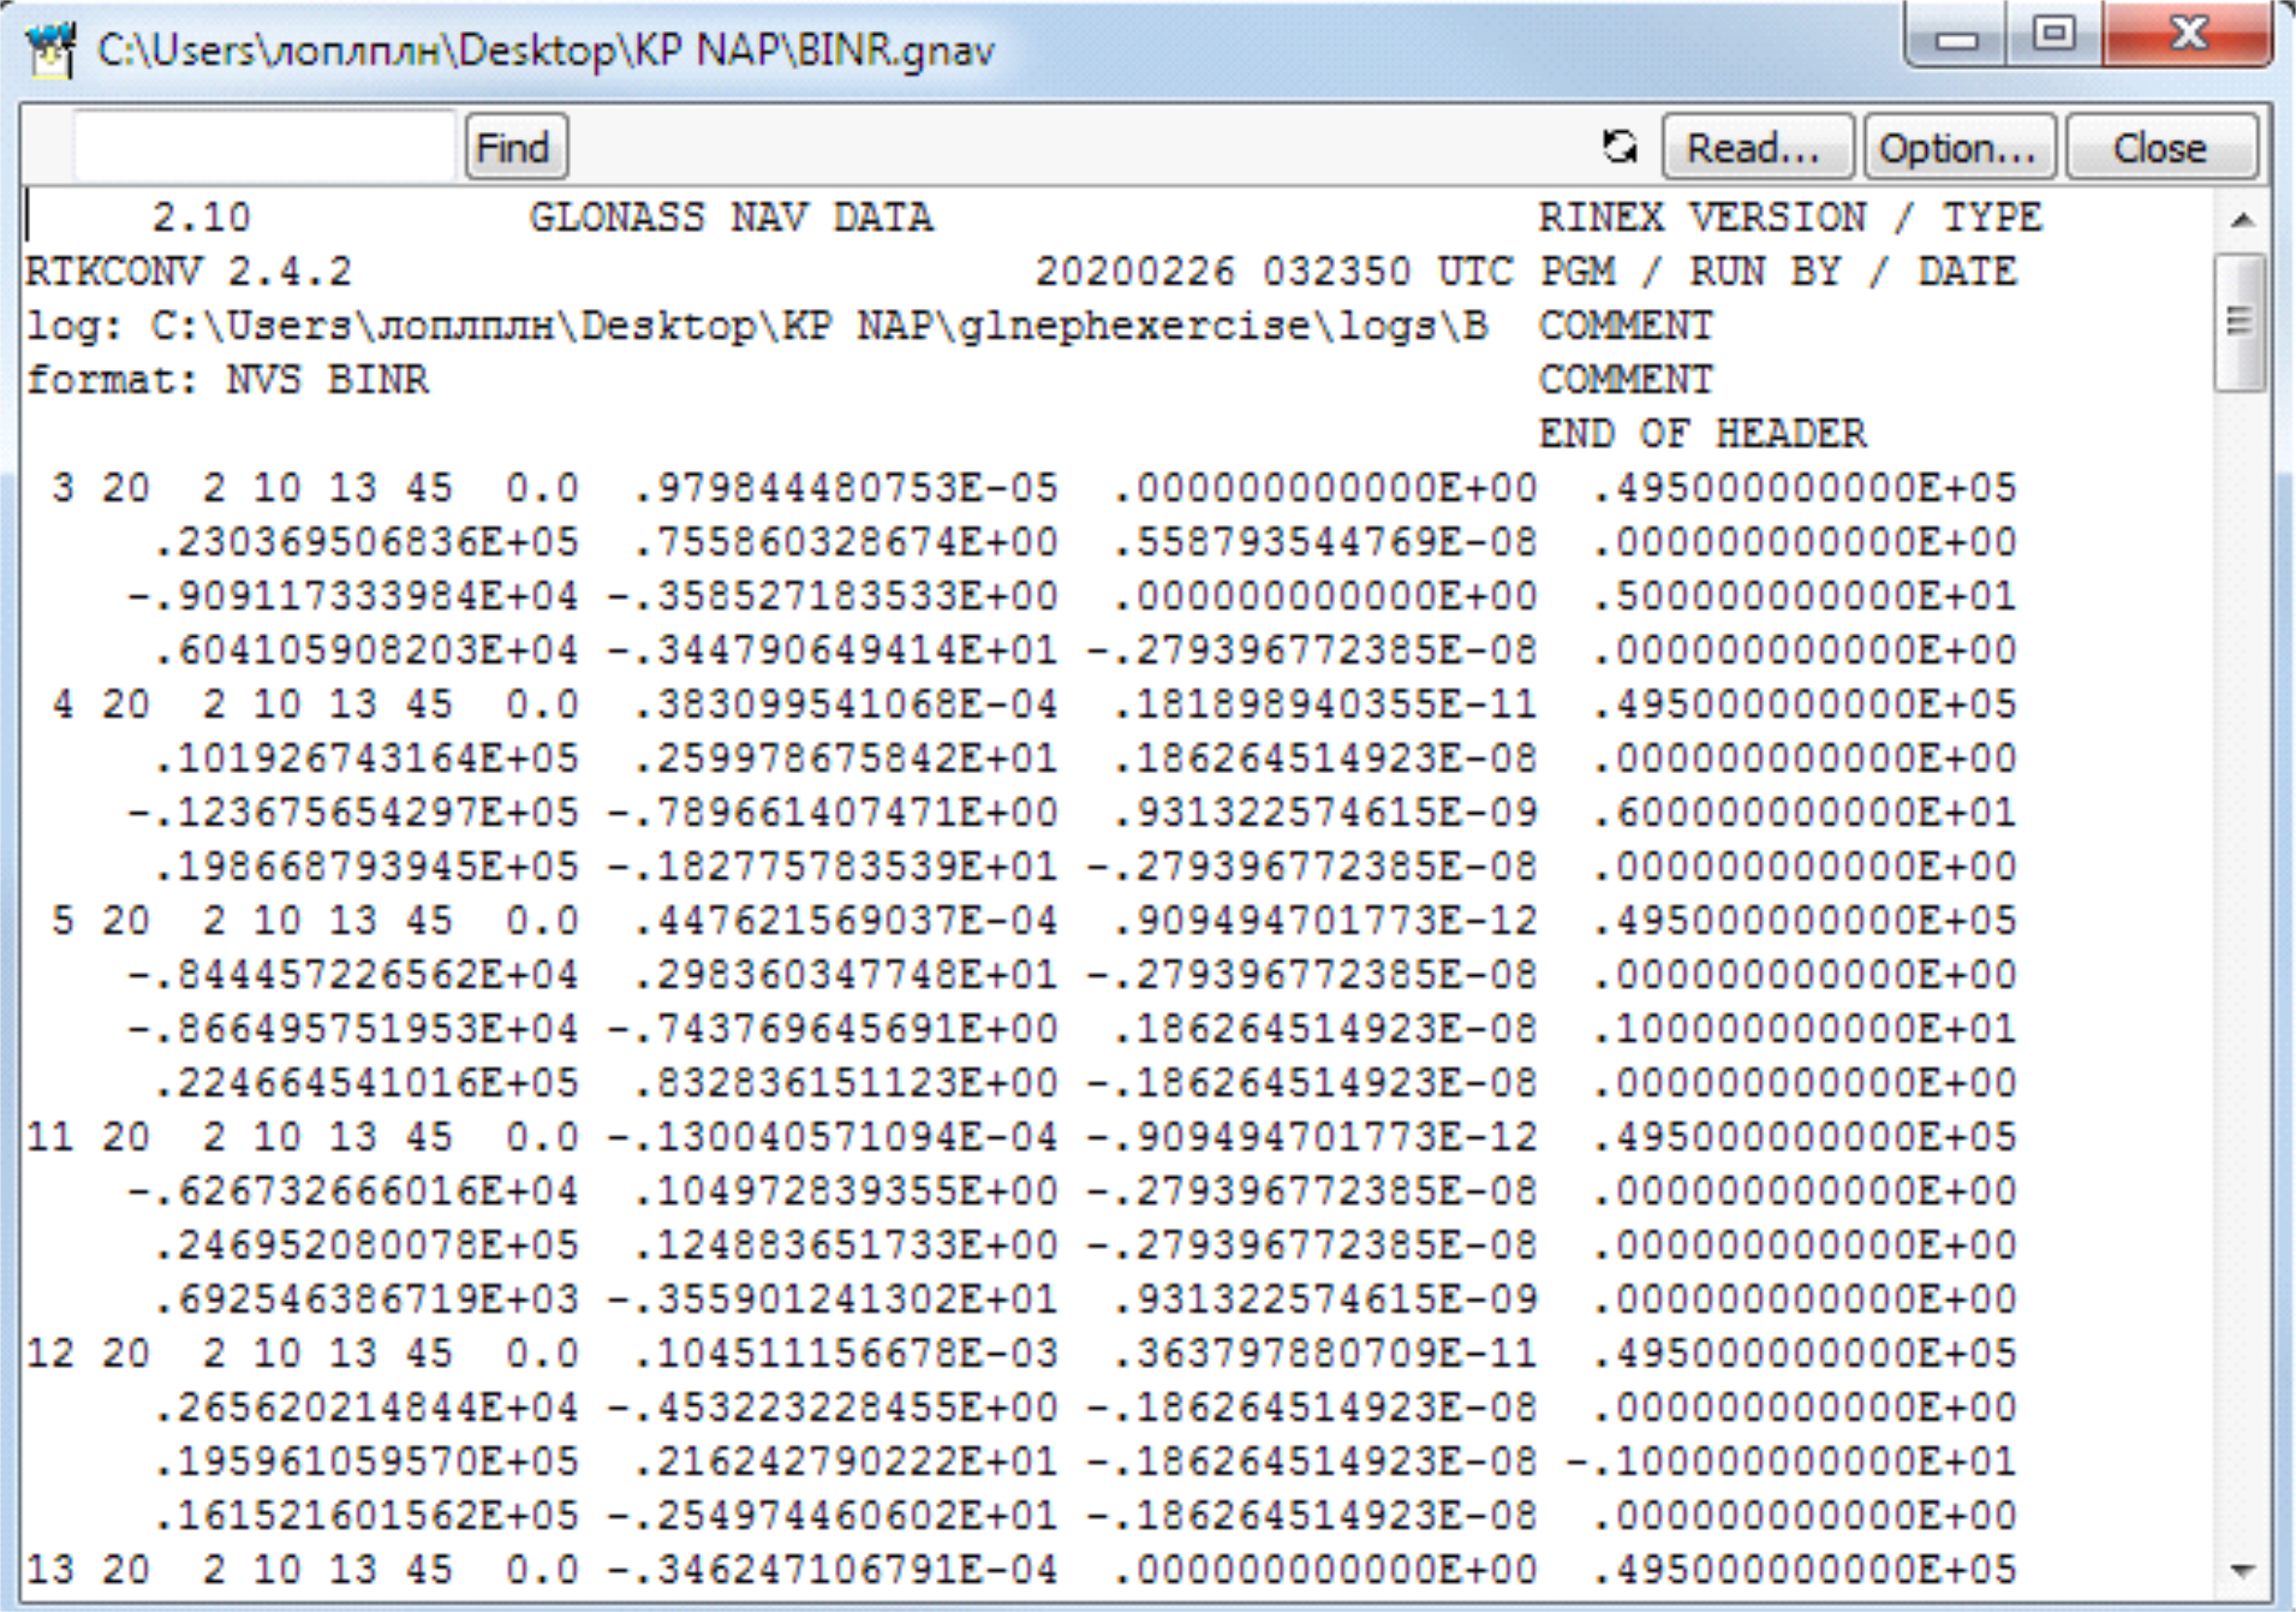
\includegraphics[scale=0.7]{efem_2}}
	\caption{Полученный файл с эфемередами}
	\label{efem_2}
\end{figure}
 
 \subsection{Получение Sky View}
 Для того что бы получить Sky View нужно зайти  на сайт https://www.gnssplanning.com/ . В разделе  «settings » установить параметры времени и места, для которых будет отображено Sky View (рис.\ref{gnss}).
 
 	\begin{figure}[h!]
 	
 	\centering{
\includegraphics[scale=0.7]{gnss}}
 	\caption{Интерфейс gnssplanning }
 	\label{gnss}
 \end{figure}




В нашем случае эти параметры равны:

Широта: N 55° 45' 24.39"

Долгота: E 37° 42' 11.53"

Высота: 150 м

День: 10.02.2020

Время начала слежения: 12.00 по UTC +00:00

Время слежения: 12 часов

Затем нужно зайти в раздел «satellite Library», выбрать систему ГЛОНАСС и оставить галочку только у «своего» спутника (рис.\ref{gnss_2}). 
 
 \begin{figure}[h!]
 	
 	\centering{
\includegraphics[scale=0.7]{gnss_2}}
 	\caption{Интерфейс gnssplanning }
 	\label{gnss_2}
 \end{figure}
 После этого можно наблюдать Sky View в разделе «Sky Plot» (рис.\ref{gnss_3}).
 
 \begin{figure}[h!]
 	
 	\centering{
\includegraphics[scale=0.7]{gnss_3}}
 	\caption{Интерфейс gnssplanning }
 	\label{gnss_3}
 \end{figure}
 Важно: данный сервис не отображает одновременно все пролеты спутника в заданном диапазоне времени.  Необходимо снять два графика в разное время (каждое соответствует своему витку) (рис. \ref{skyv_1}, \ref{skyv_2}).
 
 \begin{figure}[h!]
 	
 	\centering{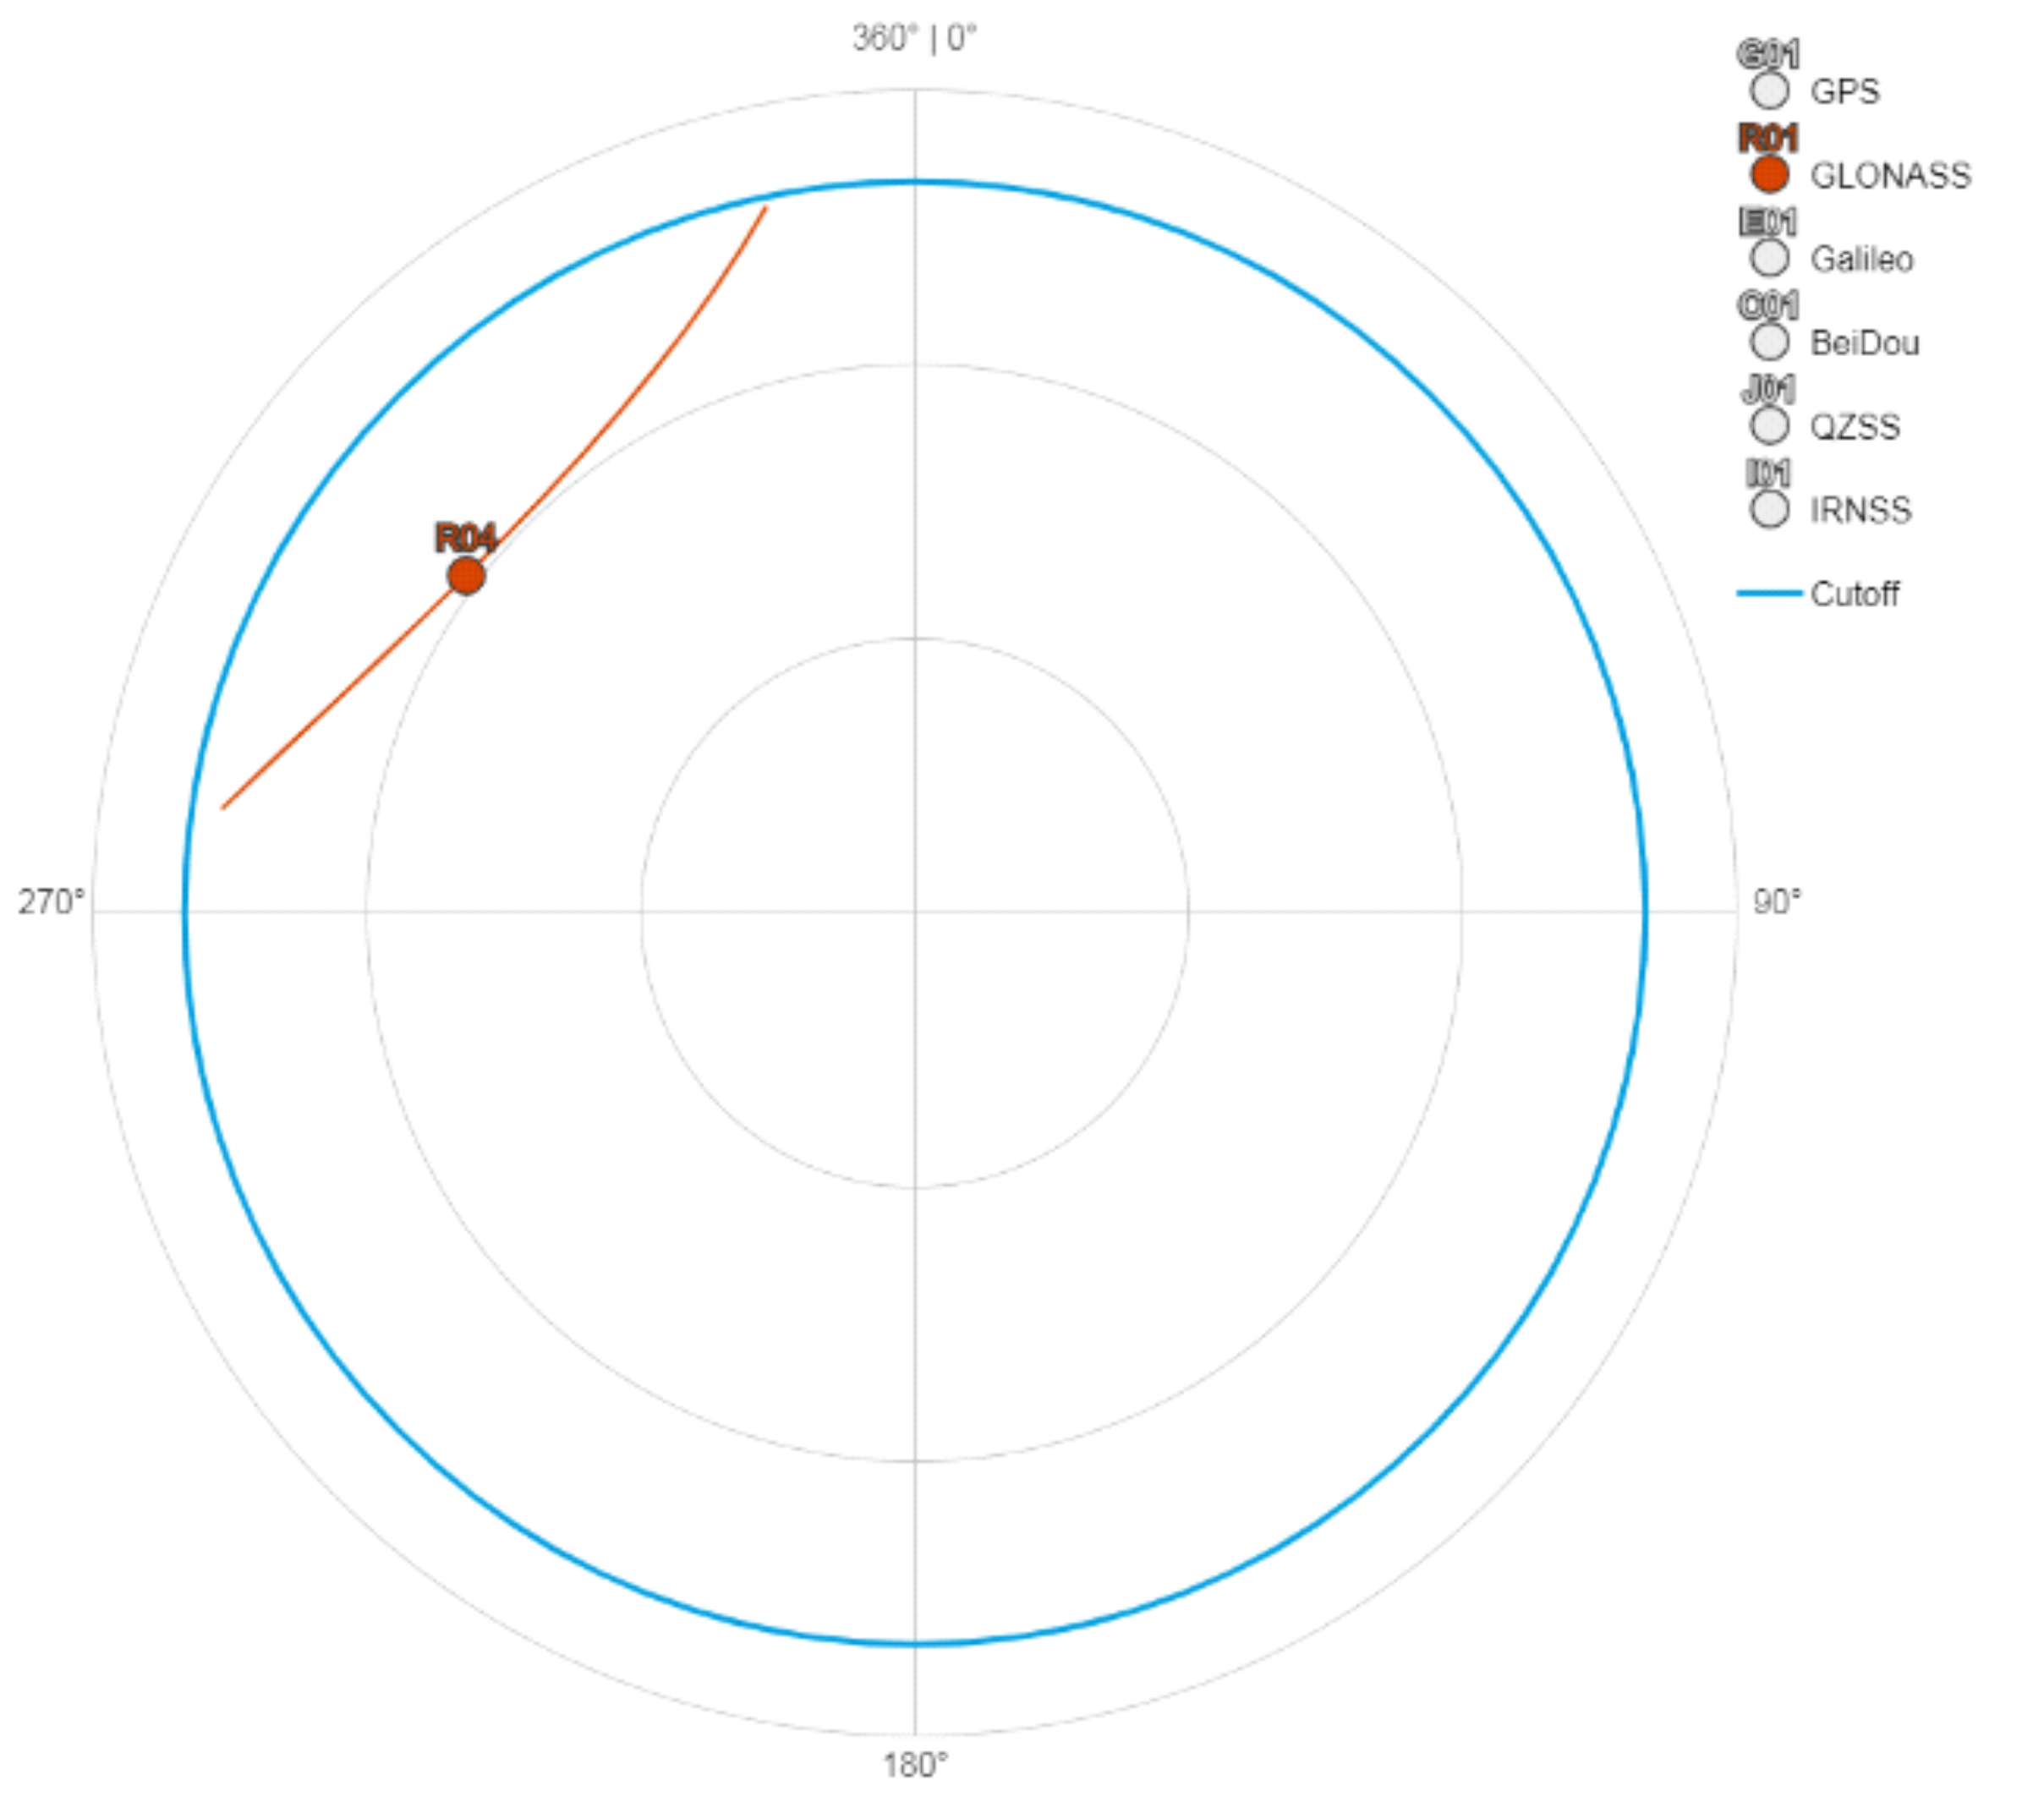
\includegraphics[scale=0.8]{skyv_1}}
 	\caption{Sky View первого витка НКА }
 	\label{skyv_1}
 \end{figure}
 \begin{figure}[h!]
	
	\centering{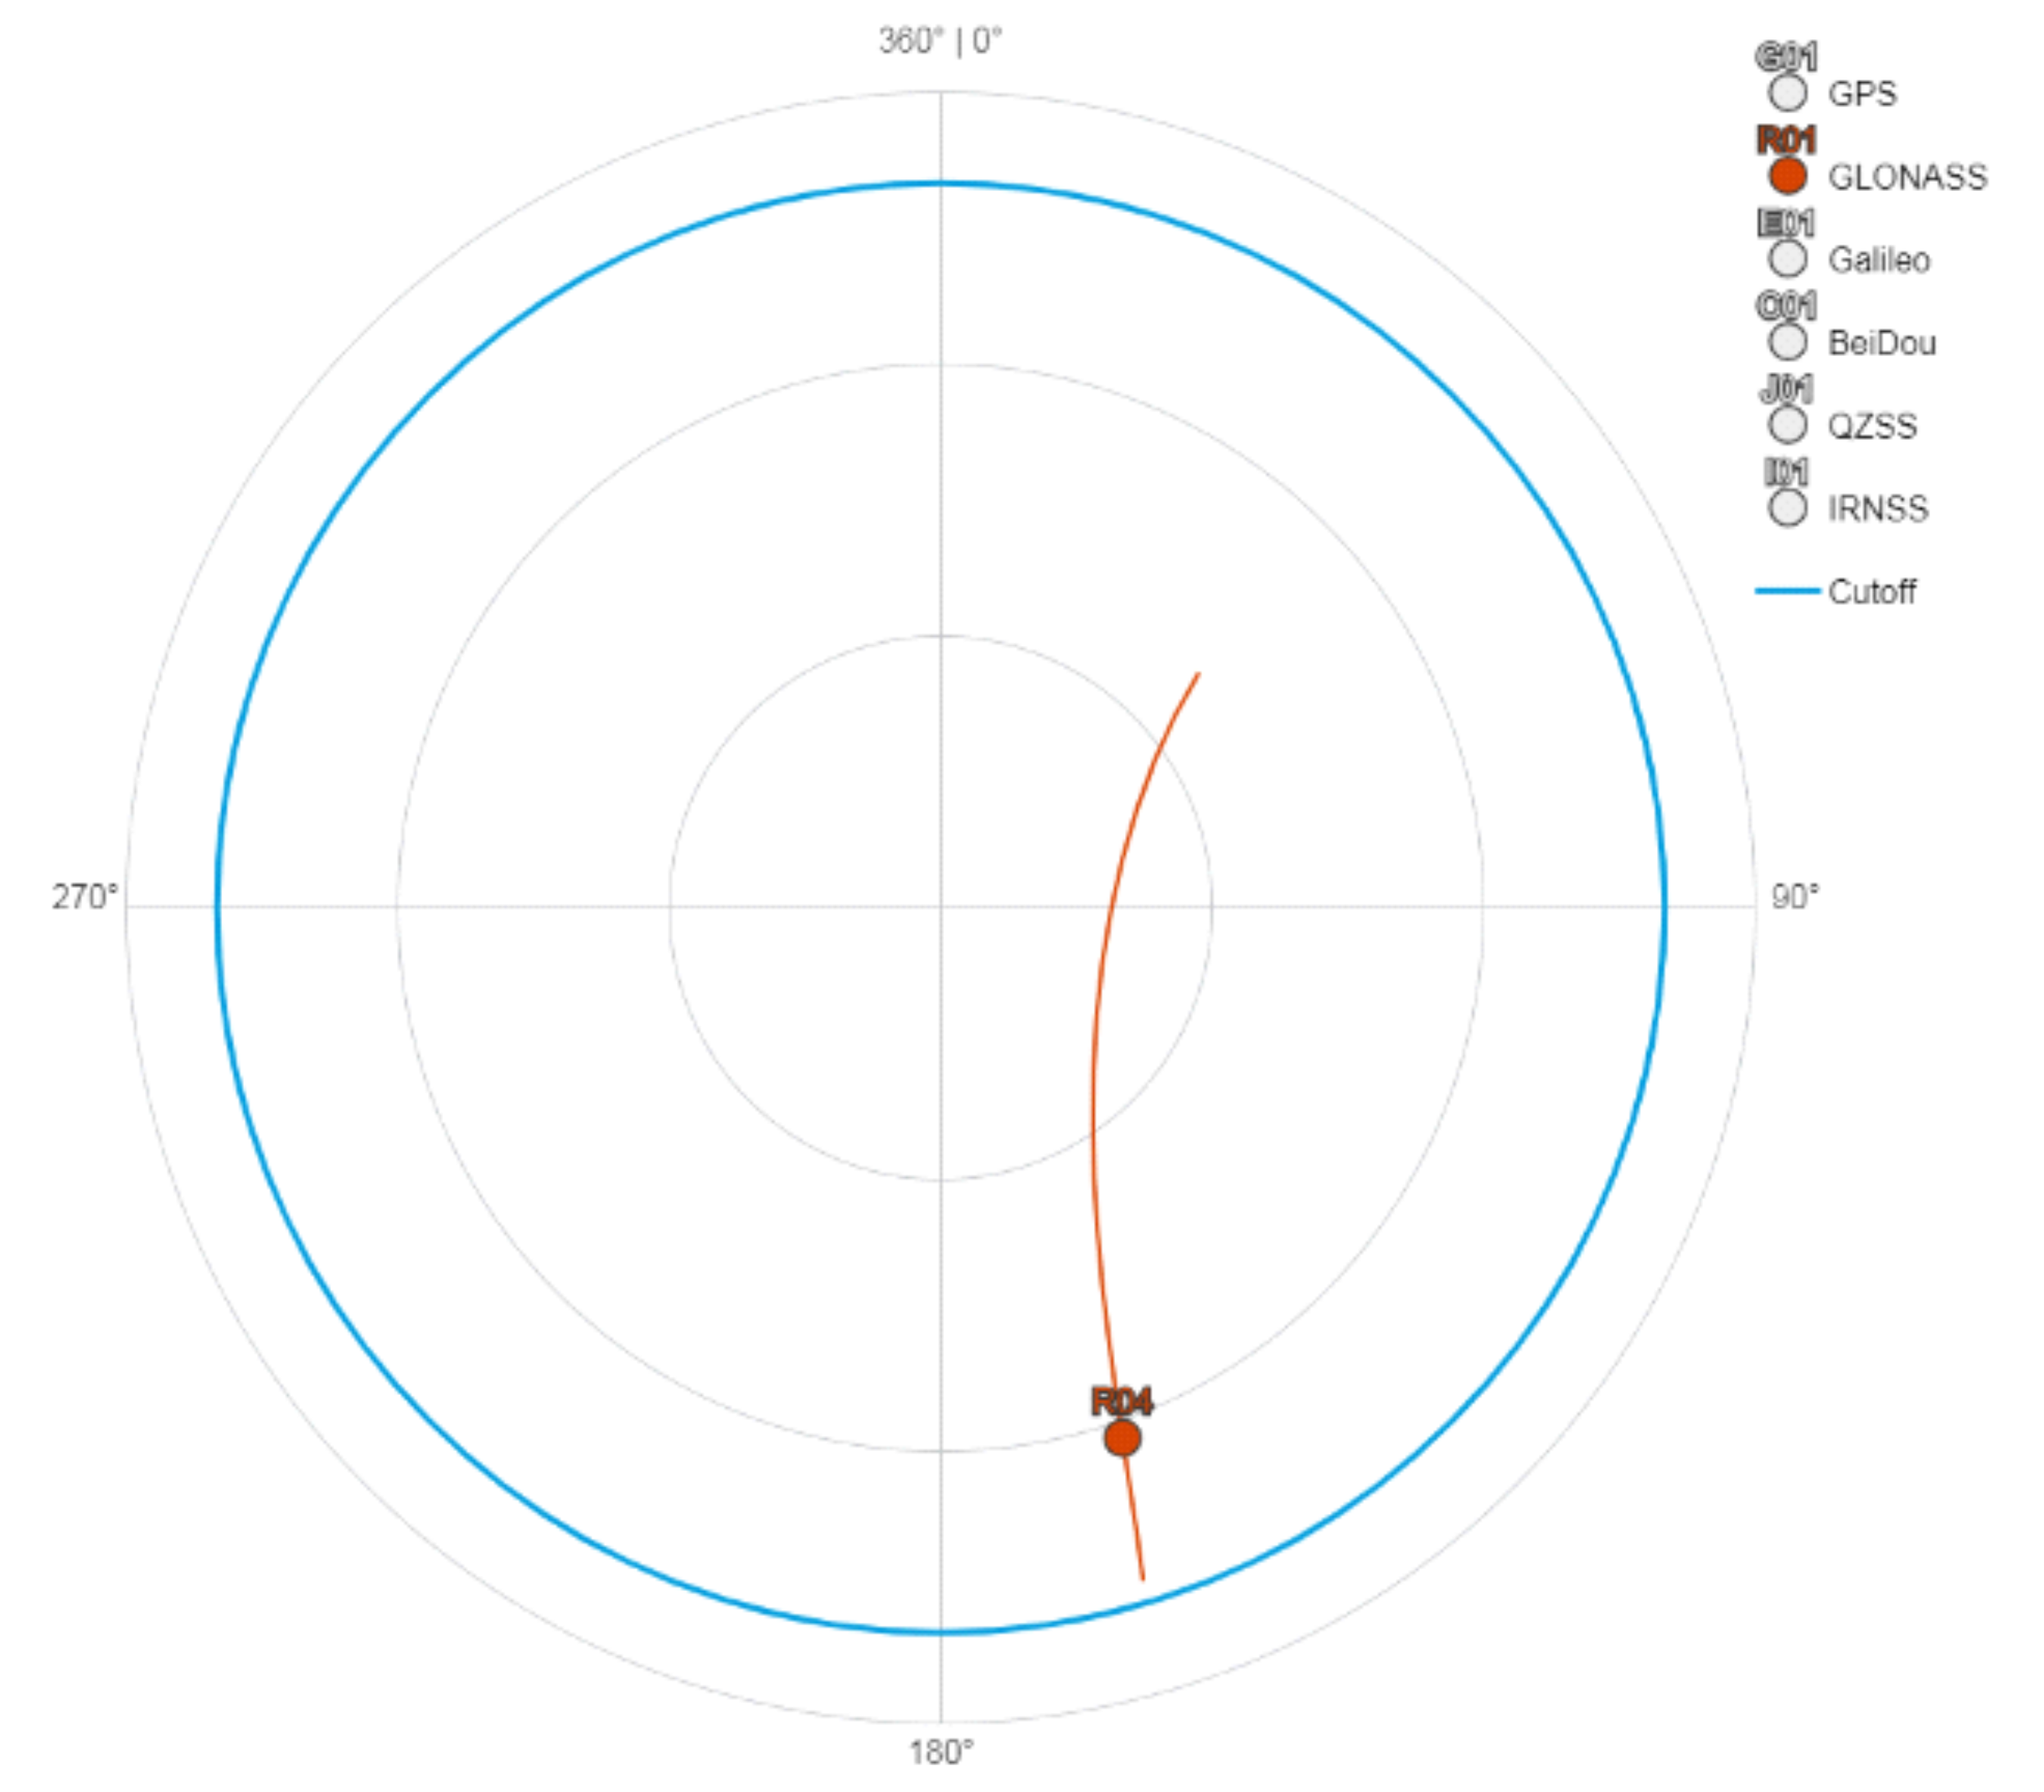
\includegraphics[scale=0.8]{skyv_2}}
	\caption{Sky View второго витка НКА }
	\label{skyv_2}
\end{figure}

\subsection{Заключение по первому этапу}
На первом этапе курсового проекта с помощью сервиса gnssplanning и пакета RTKLIB была произведена обработка данных, полученных с антенны приемника, расположенной на Е корпусе МЭИ.

По результатам обработки были получены:

- Эфемериды для НКА, наблюдаемых в заданном временном интервале;

- Файл с эфемеридой заданного НКА в формате .gnav;

- Sky View для заданного НКА в заданный промежуток времени.

\newpage
\section{Этап 2. Моделирование}
	\subsection{Задание на этап №2}
	Требуется:
	Рассчитать положение заданного спутника, по эфемеридам, полученным в предыдущем этапе, на промежуток времени от 12.00 до 24.00 МДВ 10 февраля 2020 года. 
	
	Построить модель движения КА в инерциальной СК и в СК ECEF ПЗ-90.11. 
	
	Построить SkyView за указанный временной интервал.

	\subsection{Теоретическая информация для расчета}
	В \cite{ICD} приведены формулы для расчета положения КА по данным эфемерид. Суть расчета: из уже имеющихся на момент получения эфемирид координат путем интегрирования и добавления поправок на небесные тела получают координаты спутника. Координаты можно получить как на более позднее время, так и на более раннее. При этом стоит учитывать, что с увеличением разницы во времени между временем получения эфемерид и расчетным временем, точность вычесления координат падает. В \cite{ICD} указано, что разница во времени для реального потребителя не должна превышать 15 минут.  
	
	Рассмотрим подробнее  алгоритм вычесления.
	Поскольку интегрирование осуществляется в прямоугольной абсолютной геоцентрической системе координат, а эфемеридная информация передается в системе координат связанной с Землей  ПЗ-90-02, выполнется перевод по формулам на рис.\ref{1}.
	
	\begin{figure}[h!]
		
		\centering{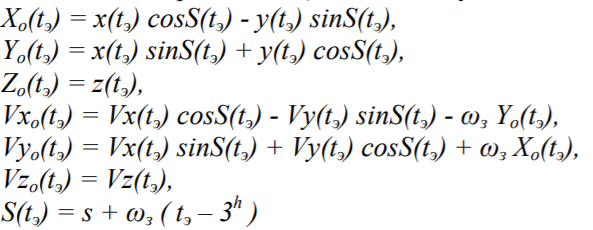
\includegraphics[scale=0.7]{1}}
		\caption{формулы перевода из СК ПЗ-90-02 в абсолютную геоцентрическую СК }
		\label{1}
	\end{figure}
	
	Полученные координаты являются начальными условиями для интегрирования. Метод интегрирования Рунге-Кутты 4 порядка, общие формулы на рис.\ref{2}.
	
	\begin{figure}[h!]
		
		\centering{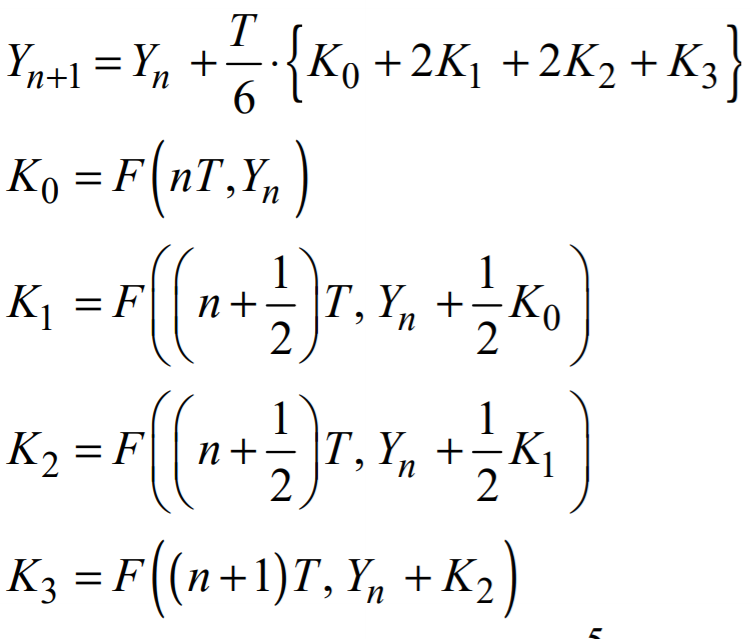
\includegraphics[scale=0.4]{2}}
		\caption{Интегрирование методом Рунге-Кутты 4 порядка }
		\label{2}
	\end{figure}
	
	
	При этом в качестве интегрируемой функции берутся выражения с рис.\ref{3}. Так же в \cite{ICD} указано, что поправки на небесные тела можно учесть однократно, если прибавить их к итоговым вычислениям, воспользовавшись формулой с рис.\ref{4}.В этом случае ошибки возрастут на не более 10\% .
	
	
	\begin{figure}[h!]
		
		\centering{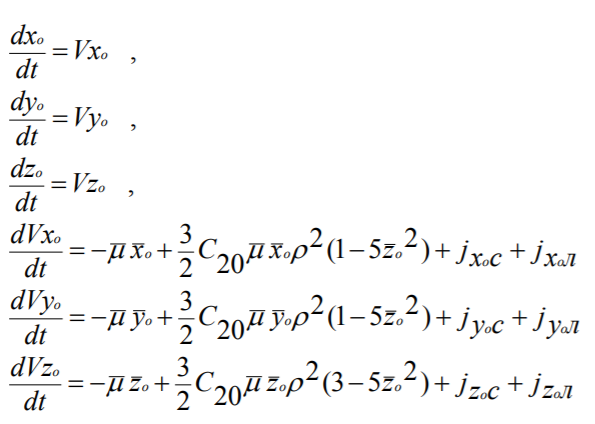
\includegraphics[scale=0.7]{3}}
		\caption{Интегрируемая функция }
		\label{3}
	\end{figure}
	
	\begin{figure}[h!]
		
		\centering{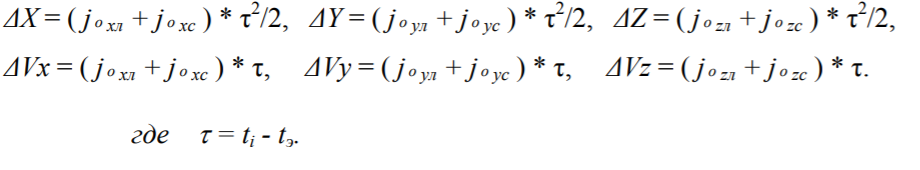
\includegraphics[scale=0.8]{4}}
		\caption{Учет поправок на небесные тела }
		\label{4}
	\end{figure}
	
	\subsection{Практическая реализация}
	
	Для практической реализации на данном этапе использовалась среда Matlab R2019b. Расчетный модуль состоит из одного скрипта, и нескольких функций. 
	В главном скрипте выполняется:
	
	1. Задание эфемиридных и временных данных, а так же констант.
	
	2. Пересчет систем координат.
	
	3. Вызов функции расчета временных параметров, вызов функции расчета координат.
	
	4. Моделирование сферы Земли и траекторий НКА по полученным данным.
	
	Всего функций, которые вызываются в данном модуле четыре.
	Первая из них, это функция "time". Поскольку функция вызывается лишь единожды, расчеты из нее можно перенести в основной скрипт, но это немного "засорит" программное поле.
	Вторая функция "math\_2" производит расчет координат на интервал времени. Ее так же можно перенести в основной скрипт. В этой функции учтены две ситуации с временным интервалом:
	первая- координаты вычисляются на моменты времени больше чем время прихода эфемерид, вторая- координаты вычисляются на время и до, и после времени прихода эфемерид. Если с первым вариантом никаких сложностей не возникает, со вторым связано появление множества "костылей" в программе. Первое что нужно учитывать, это то, что для вычесления координат на более ранее время, нужно интегрировать с шагом -dt. Поскольку вектор каждого навигационного элемента будет инвертирован во времени (т.е $ X=[x_{te}, x_{te-1},...,x_{tstart}]$), его тоже нужно повернуть на 180 градусов. 
	На рис.\ref{5} изображена концепция вычисления координат на вес временной интервал. 
	
	\begin{figure}[h!]
		
		\centering{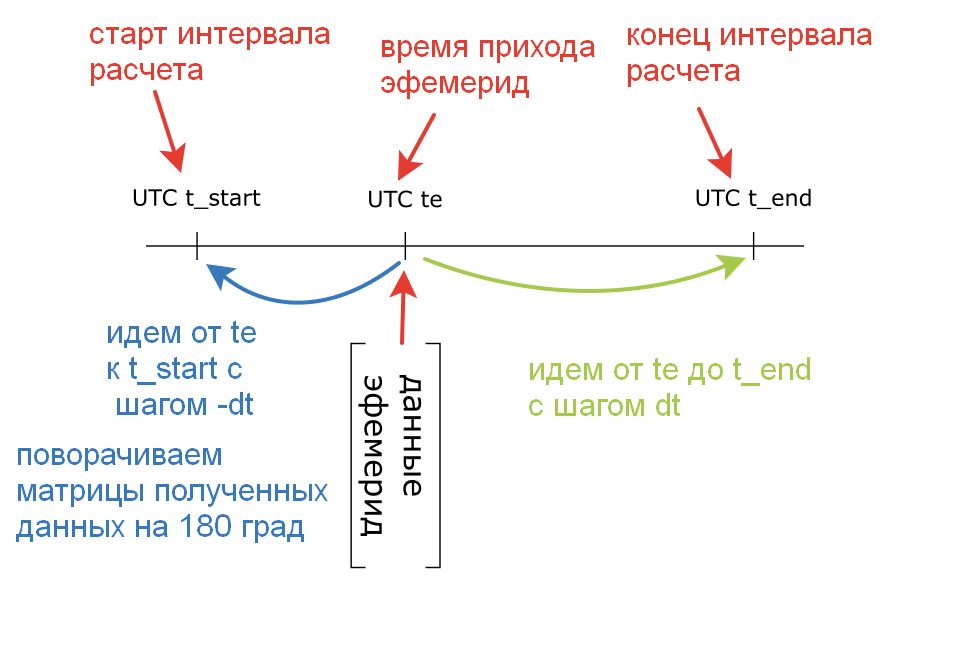
\includegraphics[scale=0.5]{5}}
		\caption{Временные интервалы }
		\label{5}
	\end{figure}
	
	Данные для двух временных интервалов вычисляются отдельно, а затем склеиваются. Для вычисления координат для каждого интервала используется функция "RungeKUTT" , которая и производит интегрирование начальных значений. Сама интегрируемая функция задана отдельно, и называется "F". Внутри нее происходят вычесления по формулам с рис.\ref{3}. 
	
	
	После того, как все вычисления выполнены, программа производит моделирование траектории движения НКА в следующих СК:
	
	1. Инерциальная;
	
	2.ПЗ-90;
	
	3.WGS84;
	
	4.Связанная с приемником (SkyVeiw).
	
	Отдельно хочется отметить, что одна из сложностей была в том, что координаты X были с инвертированным знаком, что создавало эффект "перевернутой земли".
	
	
	\subsection{Результат работы}
	В результате программы были получены следующие графики траекторий движения:
	
	1. В инерциальной СК, рис.\ref{inertz};
	
	2.В СК ПЗ-90, рис.\ref{PZ};
	
	3.В СК WGS84, рис.\ref{WGS};
	
	4.В Связанной с приемником СК (SkyVeiw), рис.\ref{skyv}
	
	
	
	\begin{figure}[h!]
		
		\centering{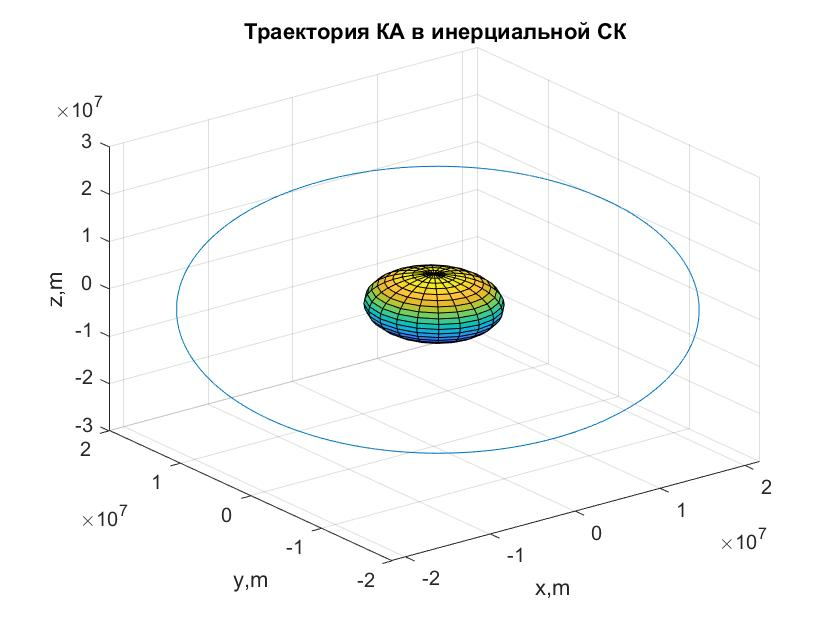
\includegraphics[scale=0.4]{inirtz}}
		\caption{Траектория движения в инерциальной СК  }
		\label{inertz}
	\end{figure}
	
	\begin{figure}[h!]
		
		\centering{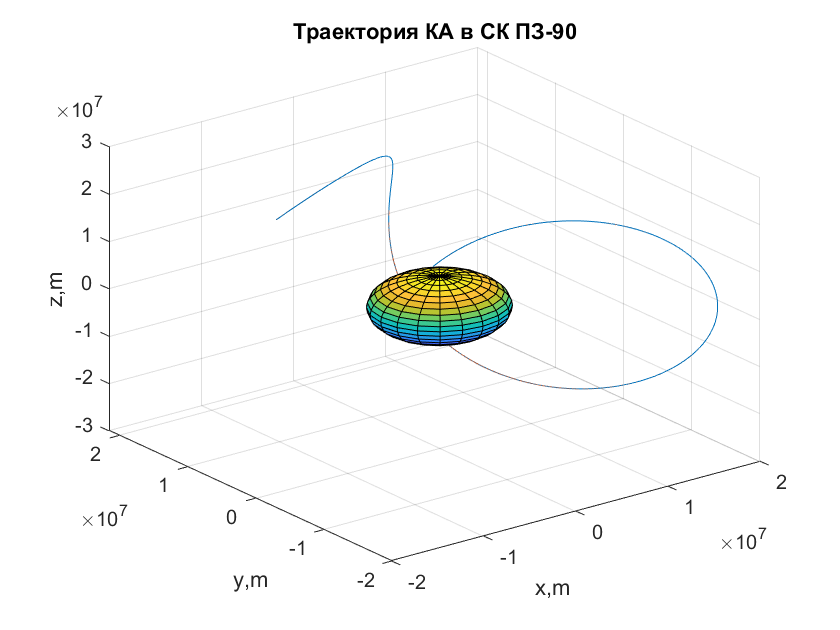
\includegraphics[scale=0.4]{PZ90}}
		\caption{Траектория движения  СК ПЗ-90 }
		\label{PZ}
	\end{figure}
	
	\begin{figure}[h!]
		
		\centering{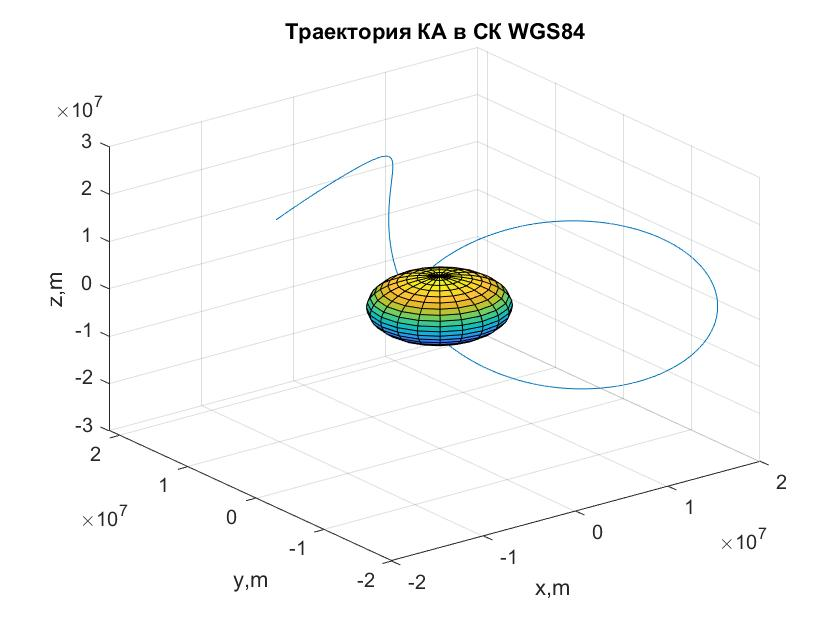
\includegraphics[scale=0.4]{WGS}}
		\caption{Траектория движения в СК WGS84  }
		\label{WGS}
	\end{figure}
	
	\begin{figure}[h!]
		
		\centering{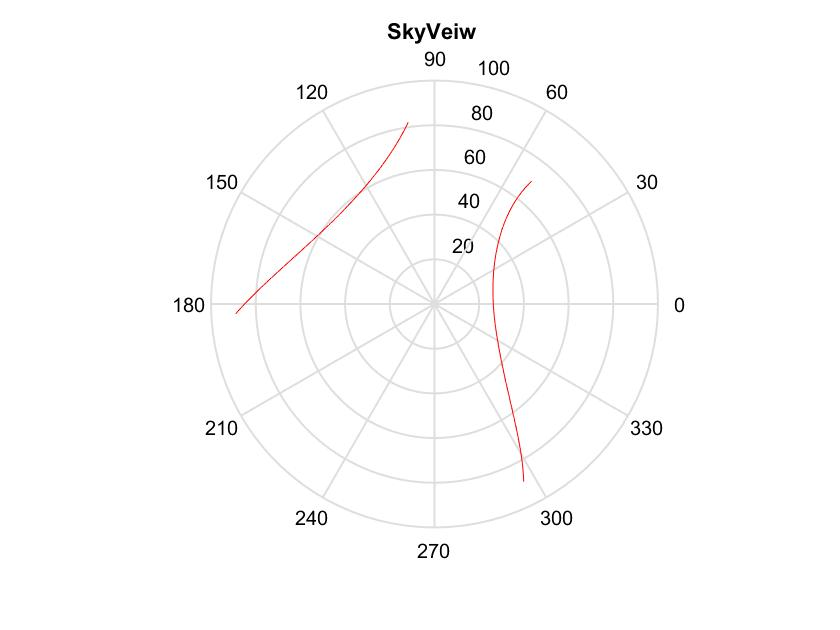
\includegraphics[scale=0.4]{skyv}}
		\caption{Траектория движения в СК связанной с приемником }
		\label{skyv}
	\end{figure}
	
	\newpage
	\subsection{Заключение по второму этапу.}
	
	На втором этапе курсового проекта были получены данные о положении НКА на промежуток времени с 12.00 по 24.00 10 февраля 2020 года. Данные эфемерид были взяты с первого этапа курсового проекта. Получены изображения траектории НКА на заданный промежуток времени. По результатам работы на этапе была получена следующая научно-техничекая продукция:
	
	-программа расчета положения НКА;
	
	-графики траекторий НКА на заданный интервал времени;
	
	- Sky View для заданного НКА в заданный промежуток времени.

\newpage	
\section{Этап 3.Реализация}
\subsection{Задание на этап №3}
Требуется:
Разработать на языке С/С++ функцию расчета положения спутника ГЛОНАСС на заданное время по шкале UTC, минимизируя время её исполнения и количество затрачиваемой оперативной памяти. Вызов функции не должен приводить к выбросу исключений или утечкам памяти при любом наборе входных данных.


\subsection{Подготовка к работе}
Для выполнения работы на данном этапе в качестве языка программирования был выбран С++. Программная среда разработки Code::Blocks 20.03. 

Необходимые для расчета входные данные можно получить из 1 и 2 этапа курсового проекта. Алгоритм реализован согласно \cite{ICD}. 

Разработчик воспользовался специальной литературой, в часности \cite{alex}, в которой достаточно подробно описаны базовые инструменты для реализации программного модуля. 
\subsection{Практическая реализация}

В практической реализации разработчик ориентировался на уже отработанный модуль, который был создан на этапе 2. Общий алгоритм работы программы не изменился, что заметно облегчало разработку модуля.Основная сложность заключалась в переходе на давно забытый разработчиком язык программирования. В связи с этим, назвать работу программы оптимальной, к сожалению, нельзя. Тем не менее, программа выполняет расчет корректно.

Модуль состоит из проекта "trynotcry", включающнего в себя несколько файлов расширения .cpp.

В файле "main.cpp" реализованы следующие действия:

1. объявление входных данных;

2. Расчет необходимых временных параметров системы ГЛОНАСС;

3. Пересчет координат в требуемый для интегрирования формат;

4. Вызов функции, которая обеспечивает непосредственно  расчет;

5. Создание текстовых файлов с координатами x, y, z для инерциальной СК и СК ПЗ-90.

Как  можно заметить, в данном модуле временные расчеты не вынесены в отдельную функцию.Причина этому- расчет временных параметров происходит однократно, а учитывая низкие навыки программирования на данном языке, создание отдельной функции нецелесообразно, что конечно не отменяет "засорение" пространства головного файла.

Как и на предыдущем этапе, самое ценное скрыто в функции с названием "math2", которая вынесена в отдельный файл .срр с идентичным названием. 

В этой функции объявляются массивы, состоящие из структур "coord". Каждая такая структура в своем наборе имеет координаты и вектора скорости НКА на определенный момент времени.

Поскольку необходмость интегрировать "в разные стороны" не отпала, в данном модуле так же присутствуют два массива- один для измерений на время предшествующее моменту получения эфемерид (after), а другой на время от прихода эфемерид до завершения прогнозирования вектора состояния НКА (bef).

Далее нулевым элементам массивов присваиваются значения положения НКА на момент прихода эфемерид. ПОсле этого для каждого массива отдельно вызывается функция "RungeKUTT", которая и производит интегрирование параметров.

Функция "RungeKUTT" описана в файле с таким же названием. 
Из-за некоторых сомнений автора во взаимодействии функций и структур, алгоритм несколько потерял в читаемости кода, по сравнению с аналогичной функцией с предыдущего этапа.

Функция "F" не претерпела значительных изменений по сравнению с этапом №2, да и сама по себе довольна простая, поэтому от ее описания автор воздержался.

Вернемся к обсуждению функции "math2". После того, как была вызвана функция "RungeKUTT", содержимое соответствующего массива измениться. Каждый элемент массива будет содержать параметры описывающие движение НКА, причем для случая с массивом "after" параметры будут соответствовать движению в положительную сторону по оси времени, а для массива "bef" в обратную.

Для того чтобы выходные данные были правильно распределены по оси времени, был реализован алгоритм, который "склеивает" данные из двух массивов в правильном порядке. Хочется отметить, что реализация данного алгоритма в этом модуле прошла куда приятнее, чем реализация в среде Matlab.

После того, как данные получены, приходит время рассчитать и добавить поправки на небесные тела, что и осуществлено внутри функции "RungeKUTT".

После того как программа отработает, в папке рядом с ней появятся 6 файлов формата .txt, котрые будут содержать координаты x,y,z для двух СК.




\subsection{Результат работы}
Для отображения результатов работы полученные текстовые файлы загружаются в программу с этапа №2. Загруженные координаты наносятся на соответствующие графики, полученные в результате моделирования.
В результате программы были получены следующие графики траекторий движения:

1. В инерциальной СК, рис.\ref{inertz};

2.В СК ПЗ-90, рис.\ref{PZ};




\begin{figure}[h!]
	
	\centering{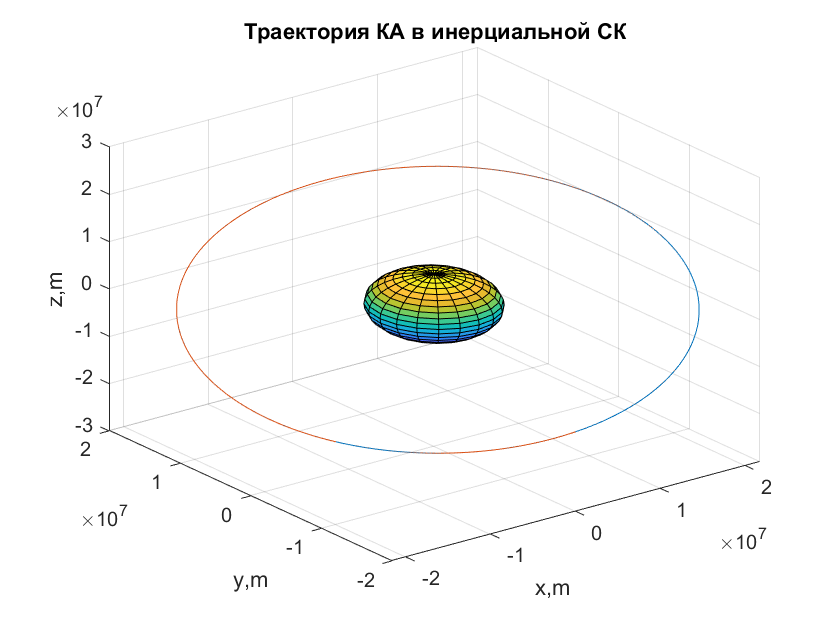
\includegraphics[scale=0.4]{inertz}}
	\caption{Траектория движения в инерциальной СК  }
	\label{inertz}
\end{figure}

\begin{figure}[h!]
	
	\centering{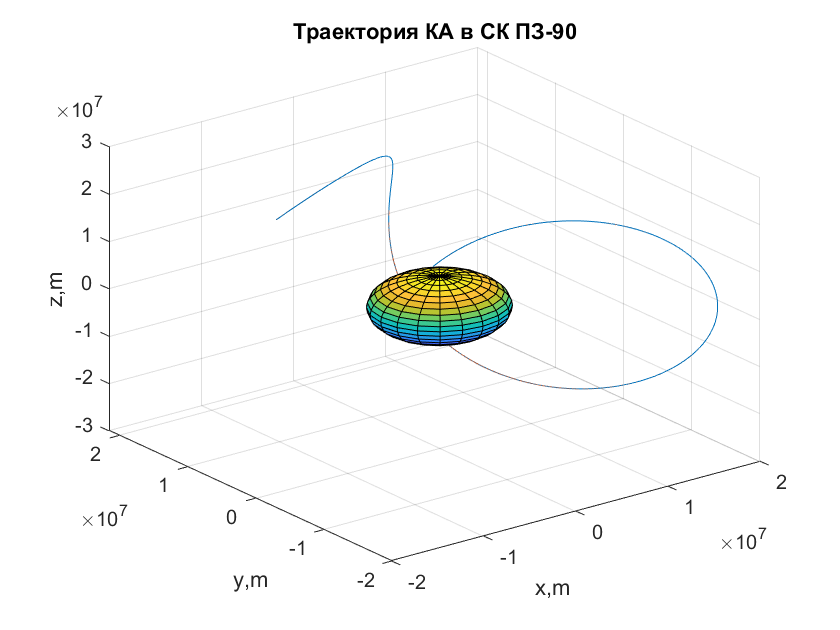
\includegraphics[scale=0.4]{PZ90}}
	\caption{Траектория движения  СК ПЗ-90 }
	\label{PZ}
\end{figure}




\subsection{Заключение по третьему этапу.}

На третьем этапе курсового проекта был разработан модуль на языке C++, позволяющий получить координаты НКА на заданный интервал времени для двух СК.  По результатам работы на этапе была получена следующая научно-техничекая продукция:

-программный модуль расчета положения НКА;

-графики траекторий НКА в инерциальной СК и в СК ПЗ90, на заданный интервал времени.

\newpage
\section{Общие выводы}
В ходе работы над данным курсовым проектом были получены следующие навыки:

- использования сервиса Trimble GNSS Planning Online;

- использования пакета RTKLIB;

- использования системы контроля версий;

- использования системы верстки Latex;

- моделирования траектории НКА в разных СК (в том числе связанных с приемником);

- реализации заданного алгоритма на языке C++.

Выводы по результатам работы над курсовым проектом:

Не стоит пренебрегать статьями и пособиями, которые повторяют смысл официальных документов, очень часто в них некоторые моменты обсуждаются подробнее. 

Этап моделирования лучше всего начинать с определения структуры будущего алгоритма, определения необходимости использования функций. Так же необходимо проверять, как те или иные переменные передаются из\ в функции.

Этап реализации и сложнее, и легче одновременно- с одной стороны, уже есть готовый алгоритм по которому можно сверить некоторые параметры, а с другой, реализация проходит в иной среде с более простым языком, из-за чего требуется больше внимания уделять объявлениям переменных, функций и т.п.

Полученная в ходе разработки научно-техническая продукция:

-модель расчета положения НКА на заданное время ппо данным его эфемерид  в системе Matlab;

- модуль расчета положения НКА на заданное время ппо данным его эфемерид  на языке С++;

\newpage
\addcontentsline{toc}{section}{\bibname}
\begin{thebibliography} {7}
	
	\bibitem{ICD} ИКД Глонасс 5.1, 2008
	\bibitem{alex} Эллайн Алекс, C++. От ламера до программера, 2015.
	
	
\end{thebibliography}

\end{document}
